\begin{definicja}[Algorytm]\label{def:algorytm}
Zbiór jednoznacznie określonych reguł lub zadań obliczeniowych prowadzących w skończonej ilości kroków do rozwiązania pewnego problemu \cite{IEEE}.\\
\end{definicja}

Określone w ten sposób zadania obliczeniowe są z reguły względem siebie niezależne. Pewne z nich mogą być wykonywane równolegle, inne -- sekwencyjnie, jedno po drugim. Wobec tego algorytm może być określony częściowo równolegle, częściowo sekwencyjnie.\\

Na podstawie niezależności zadań obliczeniowych algorytmy możemy podzielić na pięć klas \cite{APC2011}:
\begin{enumerate}
\item Algorytmy szeregowe
\item Algorytmy równoległe
\item Algorytmy szeregowo--równoległe (SPA, Serial--Parallel Algorithms)
\item Algorytmy nieszeregowo--równoległe (NSPA, Nonserial--Parallel Algorithms)
\item Algorytmy regularno-iteracyjne (RIA, Regular--Iterative Algorithms)
\end{enumerate}





\begin{definicja}[Algorytm sekwencyjny]\label{def:algorytm_sekwencyjny}
\textbf{Algorytm sekwencyjny} (rys.  \ref{fig:sequential}) jest ciągiem dokładnie sprecyzowanych zadań obliczeniowych \(T_i,\, i\in\mathbb{N}\) rozwiązujących dany problem, tj. wyznaczających dane wyjściowe na podstawie danych wejściowych. Zakłada się, że w algorytmie sekwencyjnym zadania wykonywane są przez jeden procesor.
\end{definicja}

\begin{figure}[h]
\centering
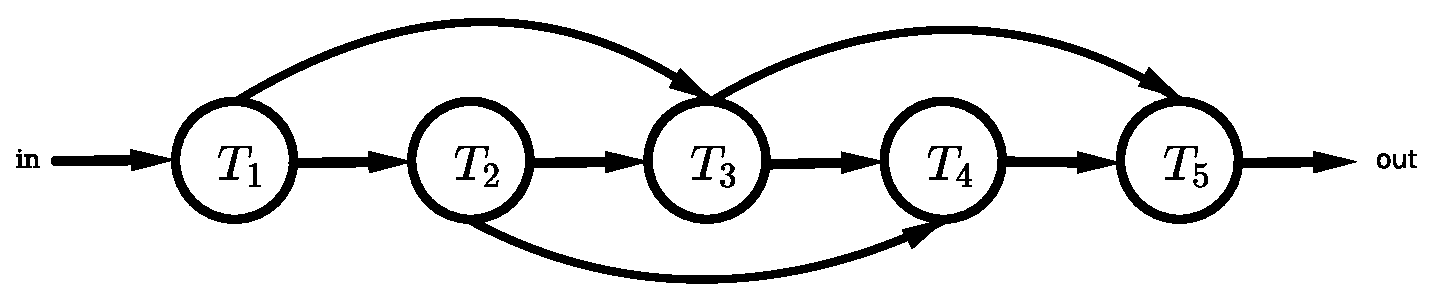
\includegraphics[width=29em]{./images/Rys2.eps}
\caption{Algorytm sekwencyjny}
\label{fig:sequential}
\end{figure}

W celu rozwiązania problemu za pomocą większej liczby procesorów należy go zdekomponować na podproblemy, które mogą być rozwiązane równolegle. Każdy z podproblemów rozwiązywany jest przez odrębny algorytm będący składową algorytmu równoległego.


\begin{definicja}[Równoległość]\label{def:rownoleglosc}
\textbf{Równoległość} w odniesieniu do oprogramowania jest to symultaniczny transfer, występowanie albo przetwarzanie poszczególnych części pewnej całości, takich jak bity składające się na znak albo znaki pewnego słowa, używając osobnych urządzeń dla ich różnych części \cite{IEEE}.
\end{definicja}

\begin{definicja}[Algorytm równoległy]\label{def:algorytm_rownolegly}
\textbf{Algorytmem równoległym} (rys.  \ref{fig:parallel}) nazywamy każdy algorytm w którym spośród określonych w nim zadań \(T_1\), \(T_2\), \(\dots\), \(T_n\) co najmniej dwa zadania \(T_i\), \(T_j\), \(i\neq j\) dzięki ich wzajemnej niezależności, mogą być wykonane równocześnie \cite{APC2011}.\\
\end{definicja}

\begin{figure}[h]
\centering
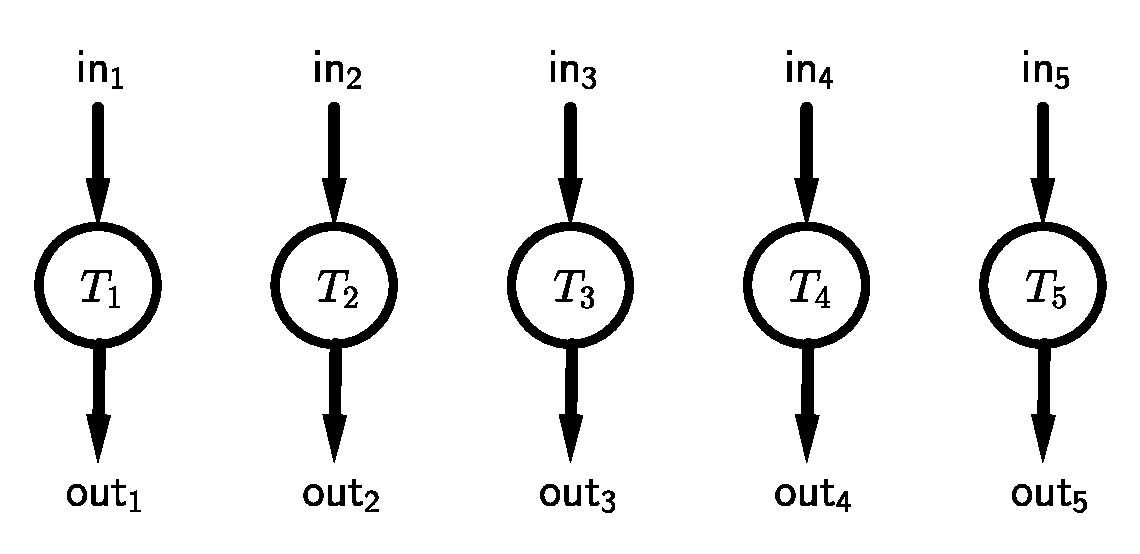
\includegraphics[width=23em]{./images/Rys1.eps}
\caption{Algorytm równoległy}
\label{fig:parallel}
\end{figure}

\begin{definicja}[Architektura równoległa]\label{def:arch_rownolegla}
\textbf{Architektura równoległa} jest to architektura wieloprocesorowa, na której można wykonywać przetwarzanie równoległe \cite{IEEE}.
\end{definicja}

Algorytmy równoległe i architektury równoległe są ze sobą blisko spokrewnione. Równoległość może być zaimplementowana na wielu poziomach używając technik sprzętowych i programowych\cite{APC2011}
\begin{enumerate}
\item{Równoległość na poziomie danych (\emph{Data-level parallelism}), gdzie pracujemy na wielu bitach danych lub na wielu danych jednocześnie.}
\item{Równoległość na poziomie instrukcji (\emph{Instruction-level parallelism}, ILP), gdzie jednocześnie procesor może wykonać więcej niż jedną instrukcję.}
\item{Równoległość na poziomie wątków (\emph{Thread-level parallelism}, TLP). Wątem jest częścią programu, która współdzieli zasoby procesora z innymi wątkami. W TLP wiele programowych wątków jest uruchamianych jednocześnie na jednym bądź wielu procesorach.}
\item{Równoległość na poziomie procesów (\emph{Process-level parallelism}). Proces to program, który jest uruchomiany na komputerze. Rezerwuje on własne zasoby komputera, takie jak przestrzeń pamięciową i rejestry.}
\end{enumerate}

\begin{przyklad}
Prostym przykładem algorytmu równoległego jest serwer siecowy, który każde zapytanie przychodzące przetwarza niezależnie od innych zapytań. Innym przykładem są wielozadaniowe systemy operacyjne, radzące sobie z jednoczesną obsługą kilku uruchomionych programów.
\end{przyklad}
%
%\begin{definicja}[Algorytmy szeregowo--równoległe]
%
%\end{definicja}
%
%\begin{definicja}[Algorytmy nieszeregowo--równoległe]
%\end{definicja}
%
%\begin{definicja}[Algorytmy regularno--iteracyjne]
%Algorytmy tej klasy reprezentowane za pomocą grafów zależności wyrażają pewien pewien ustalny schemat postępowania.
%\end{definicja}